\documentclass[12pt]{article}
\usepackage{amsmath}
\usepackage{mathtools}
\usepackage{bigints}
\usepackage{parskip}
\usepackage{amssymb}
\usepackage{relsize}
\usepackage{fullpage}
% \DeclareMathSizes{12}{17.28}{9}{7} % (a)

\DeclareMathSizes{12}{17.28}{12}{12} % (a)


\usepackage{hyperref}



	\addtolength{\topmargin}{-.5in}
	\addtolength{\textheight}{1.75in}



    \newenvironment{myindentpar}[1]%
     {\begin{list}{}%
             {\setlength{\leftmargin}{#1}}%
             \item[]%
     }
     {\end{list}}

\begin{document}
\title{College Algebra: Module 1 Definitions and Property Sheet}
\date{1-21-15}
\author{}
\maketitle


\section{Language, Notation, and Numbers of Mathematics (R.1)}

\textbf{Rational Number} - a \textit{rational number} is the ratio of two integers provided that the denominator is some integer other than 0

\textbf{Irrational Number} - a \textit{irrational number} is a number that is not rational

\textbf{Order of Operations: (PEMDAS)}
\begin{enumerate}

\item \textbf{Parentheses} - Simplifiy exressions within any parantheses or brackets beginning with the innermost grouping. If a fraction bar is used, simplify the numerator and denominator separately.
\item \textbf{Exponents} - Evaluate all exponents and roots
\item \textbf{Multiplication \& Division} - Compute multiplications/divisions in the order they occur from left to right
\item \textbf{Addition \& Subtraction} - Compute additions/subtractions in the order they occur from left to right

\end{enumerate}

\section{Algebraic Expressions and the Properties of Real Numbers (R.2)}

\textbf{Properties of Real Numbers:}

\begin{enumerate}

\item \textbf{Associative Property}

\begin{enumerate}

\item Addition: $(a+b) + c = a+ (b + c)$

\item Multiplication: $(a \cdot b) \cdot c = a \cdot (b \cdot c)$

\end{enumerate}

\item \textbf{Commutative Property}

\begin{enumerate}

\item Addition: $a+b = b + a$

\item Multiplication: $a \cdot b = b \cdot a$

\end{enumerate}

\newpage

\item \textbf{Identity Property}

\begin{enumerate}

\item Addition: $a+0 = a$

\item Multiplication: $a \cdot 1 = a$

\end{enumerate}

\item \textbf{Inverse Property}

\begin{enumerate}

\item Addition: $a+ -a = 0$

\item Multiplication: $a \cdot \dfrac{1}{a} = 1$

\end{enumerate}

\item \textbf{Distribution Property:} $a \cdot (b+c) = a \cdot b+a \cdot c$

\end{enumerate}

\section{Exponents, Scientific Notation, and a Review of Polynomails (R.3)}

\textbf{Properties of Exponents:}

\begin{enumerate}

\item \textbf{Zero Exponent Propert:} $a^0 = 1$ (provided $a \neq 0)$
\item \textbf{Negative Exponent Property:} $a^{-n} = \dfrac{1}{a^{n}}$
\item \textbf{Product Property:} $a^{m} \cdot a^{n} = a^{m+n}$
\item \textbf{Quotient Property:} $\dfrac{a^{m}}{a^{n}} = a^{m-n}$
\item \textbf{Power Property:} $(a^{m})^{n} = a^{m \cdot n}$
\item \textbf{Product to Power Property:} $(a^{m} \cdot b^{n})^{p} = a^{m \cdot p} \cdot b^{n \cdot p} $
\item \textbf{Quotient to Power Property:} $\Big(\dfrac{a^{m}}{b^{n}}\Big)^{p} = \dfrac{a^{m \cdot p}}{b^{n \cdot p}}$

\end{enumerate}

\textbf{FOIL Method:}

\centerline{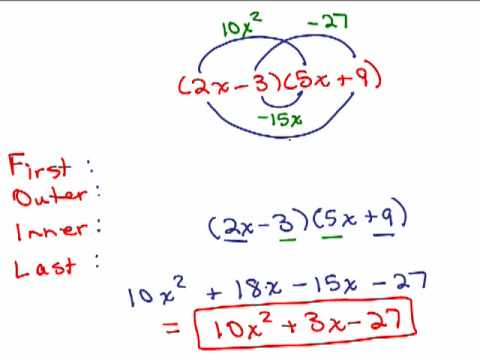
\includegraphics[scale = 0.5]{foil.jpg}}

\section{Radicals and Rational Exponents (R.4)}

\textbf{Rational (Fractional) Exponents:} $(\sqrt[n]{a})^{m} = \sqrt[n]{a^{m}} = a^{m/n}$

\textbf{Radical Properties:}

\begin{enumerate}

\item \textbf{Product Property:} $\sqrt[n]{ab} = \sqrt[n]{a} \cdot \sqrt[n]{b}$
\item \textbf{Quotient Property:}$\sqrt[n]{\dfrac{a}{b}} = \dfrac{\sqrt[n]{a}}{\sqrt[n]{b}}$

\end{enumerate}












\end{document}